\chapter{\label{ch:1-intro}Introduction} 

%\minitoc

\section{Overview}
Multiple myeloma accounts for 1-2\% of all cancers and has the second highest incidence of hematological malignancies, after non-Hodgkin’s lymphoma \cite{international2003criteria}.

% 1
\section{The adaptive immune system}
Humans are exposed to millions of potential pathogens every day and therefore require defences to be able to protect themselves against infection. These defences can be innate or adaptive. An example of an innate defence is the skin acting as a physical barrier between the outside world and the body. Another example of an innate defence is non-specific engulfing (phagocytosis) of foreign pathogens by macrophages (a type of white blood cell). Innate responses are relied upon as the first line of defence, however sometimes a more sophisticated, specialised response is required- called the adaptive immune response. (REF-mol biology of the cell).

Adaptive immune responses are specific to the pathogen that induced the response and are dependent on B cells and T cells, two major classes of lymphocytes (a class of white blood cell).
Two classes of adaptive immune responses exist: antibody responses, co-ordinated by B cells, and cell mediated immune responses, co-ordinated by T cells.
T-cell-mediated immune responses recognise foreign antigens (antibody generators; substances capable of eliciting an immune response by stimulating B or T cell activation) on the surface of cells and can either kill the pathogen-infected cells or stimulate B cells or phagocytes to help eliminate the pathogen.
In antibody responses, B cells and plasma cells secrete antibodies, also known as immunoglobulins.
Immunoglobulins are large Y-shaped proteins, which recognise and bind to the specific foreign antigen on the pathogen which stimulated their production.
Binding of immunoglobulins to antigens renders the virus or microbial toxin inactive as it blocks their ability to bind to host cells.
Additionally, antibody binding makes it easier for phagocytic cells to ingest the pathogen.
%%%%%%


%2
\subsection{Plasma cells}
%3
\subsubsection{Plasma cell development}
Stem cells are precursor cells which can give rise to at least one type of differentiated (mature) cell, with the capability of indefinite self-renewal.
Hematopoietic stem cells (HSC) are stem cells that give rise to all the cells of the hematopoietic system.
Two predominant cell populations are produced by HSCs: the common myeloid progenitor (CMP) and the common lymphocyte progenitor (CLP).
CMP differentiation produces erythrocytes (red blood cells), mast cells, monocytes, macrophages, neutrophils, eosinophils, basophils and myeloid dendritic cells.
CLP differentiation results in B cells, T cells, natural killer (NK) cells and lymphoid dendritic cells.

%% Immune cell figure
\begin{figure}
\centering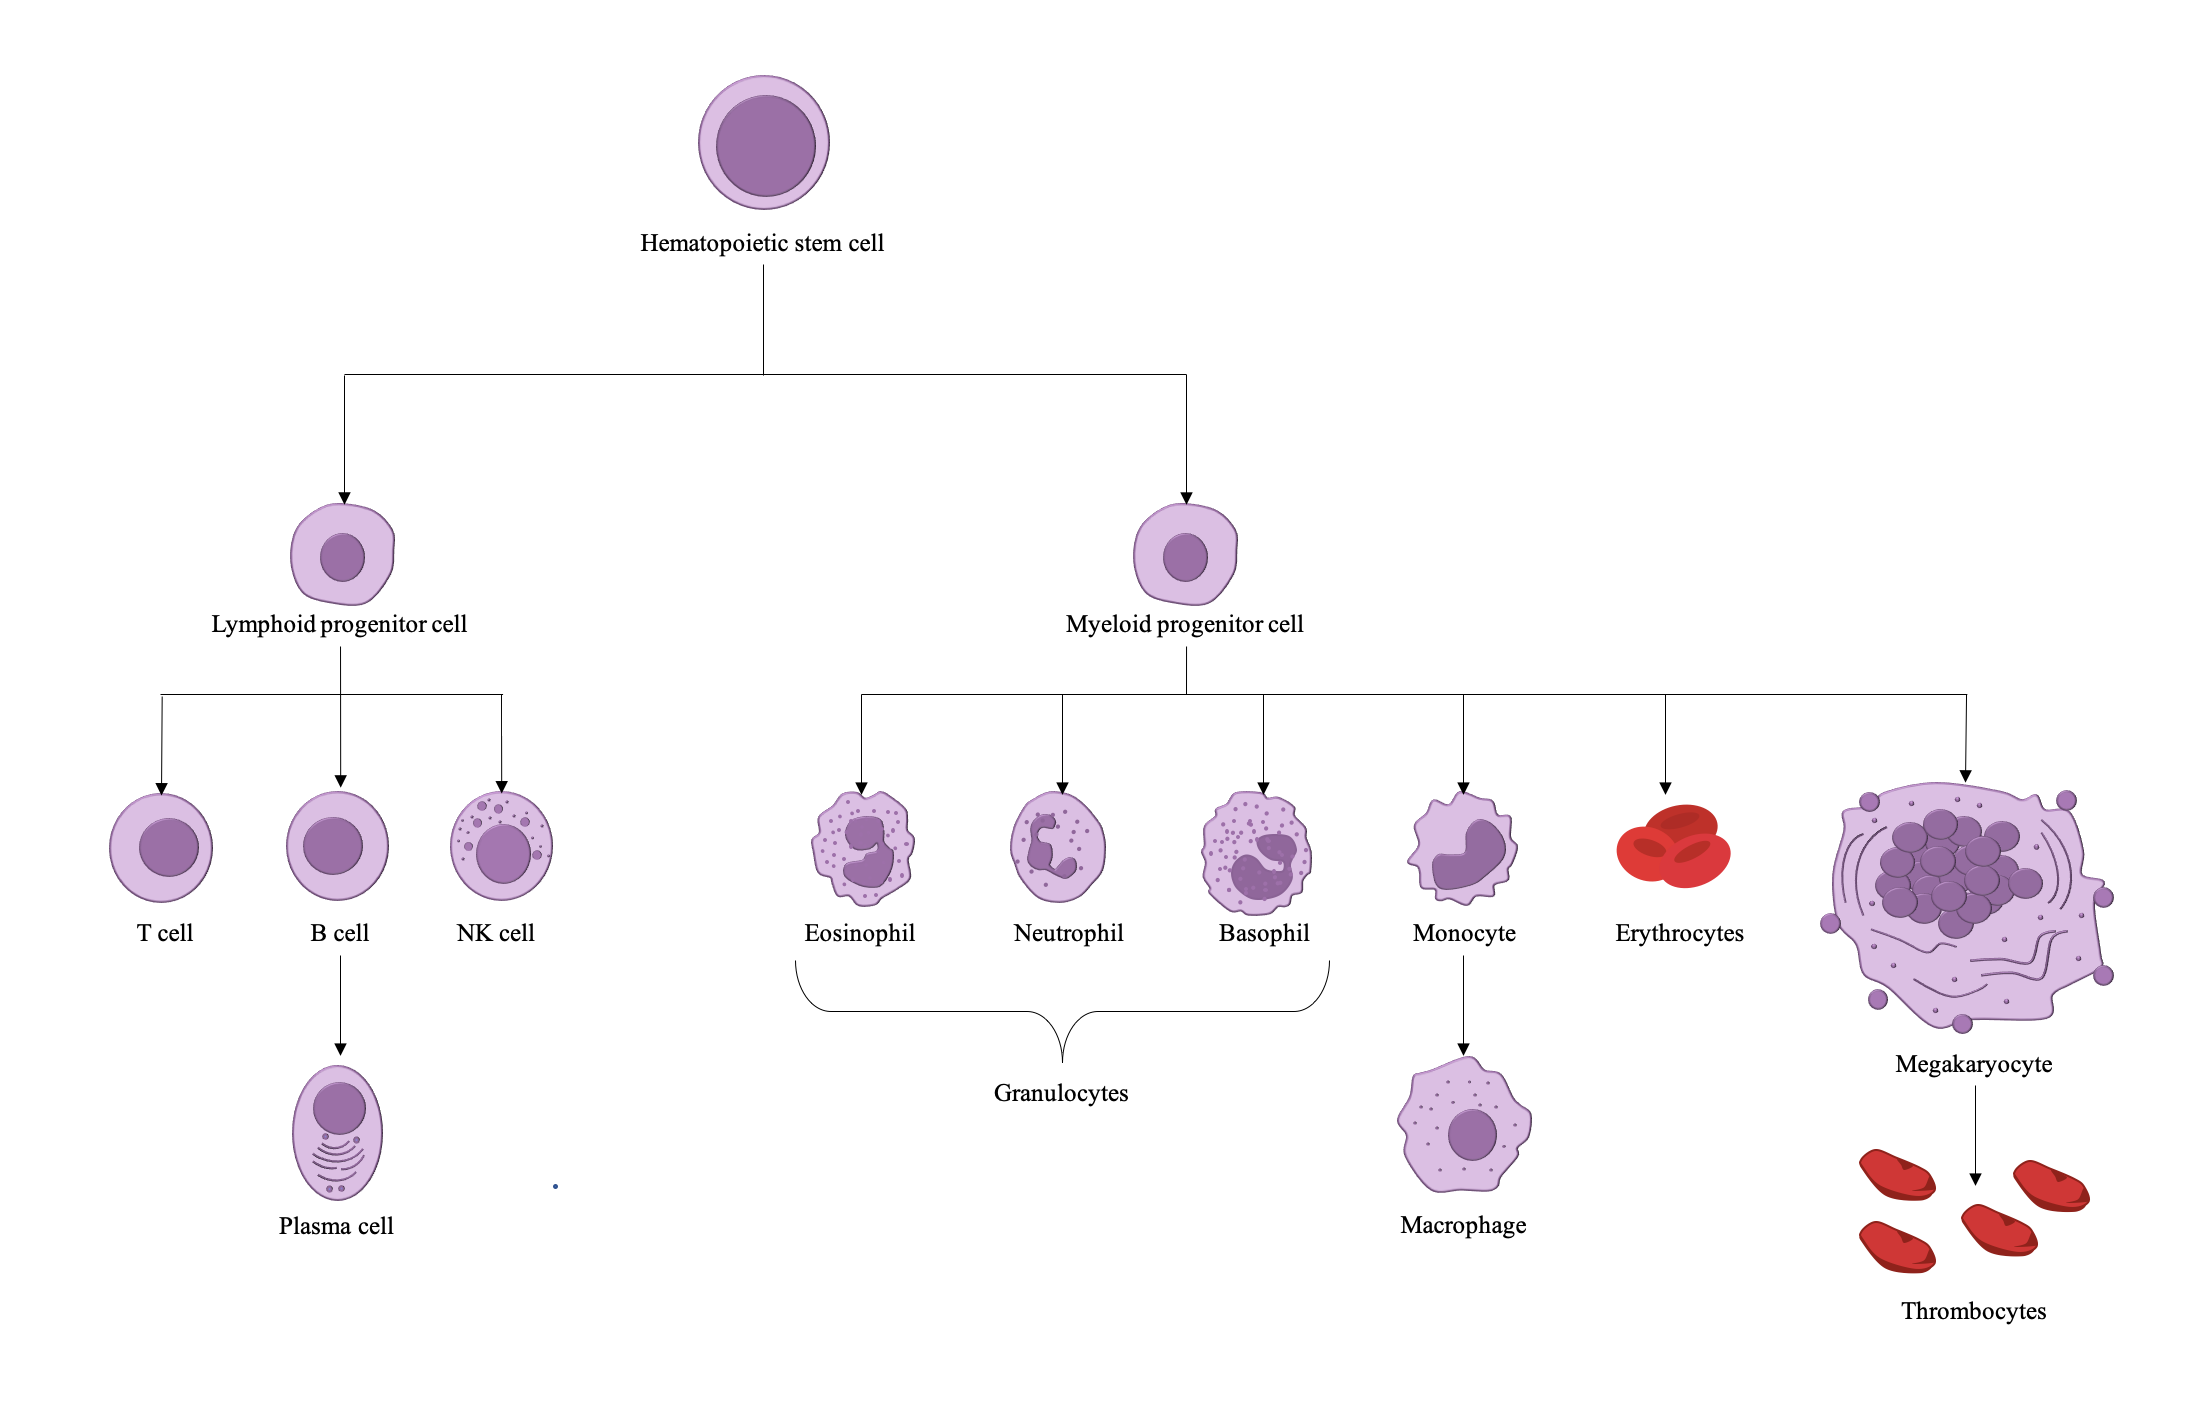
\includegraphics[width=0.7\textwidth]{figures/Introduction/immune_cells.png}
\caption[Hematopoietic system cell differentiation]{Hematopoietic stem cell (HSC) cell differentiation. HSCs divide into myeloid or lymphoid progenitor cells. Dendritic cells and a number of precursor states have been ommitted. }
\label{fig:HSC_differentiation}\end{figure}
%%

Most B cells die in the bone marrow soon after developing, however some will develop in the bone marrow, where initial stages of maturation occur and then migrate to secondary lymphoid organs, such as the spleen. Within secondary lymphoid organs, numerous critical decisions on B cell fate are made, involving complex transcriptional networks, cell interactions, gene rearrangements, and mutations (roth2014tracking; jourdan2011characterization). Terminally differentiated plasma cells are the final effectors of the B cell lineage, each dedicated to secreting large amounts of a single type of antibody. Plasma cells have an extensive rough endoplasmic reticulum (ER), and have numerous genes involved in immunoglobulin secretion upregulated, including XBP-1 and CHOP (shapiro2004plasma), to enable the production of the copious amounts of antibody required.



%1
\section{Clinical MM}

%2
\subsection{Epidemiology}
Multiple myeloma accounts for 1-2\% of all cancers and has the second highest incidence of hematological malignancies, after non-Hodgkin's lymphoma\cite{international2003criteria}.
MM is rare in individuals under the age of 40, with the average age at time of diagnosis centering around 70\cite{tsang2019multiple, palumbo2011multiple}.
MM is more prevalent in males than females and is around twice as common in black populations than in Caucasian or Asian populations\cite{nhsmyeloma}.
The average incidence rate is approximately 1-6 cases per 100000 individuals\cite{tsang2019multiple, palumbo2011multiple, teras20162016}, with the highest age-standardised incidence rates in the regions of Australasia, North America, and Western Europe\cite{cowan2018global}.
Five-year survival rate of MM patients is approximately 49\%, whilst approximately a third of MM patients survive ten years or greater\cite{cancerresearchuk, siegel2016cancer}.
%While there have been many successful medicines developed for myeloma, they all suffer from the development of drug resistance.

%2
\subsection{Presentation}
%3
\subsubsection{Precursor states}
All cases of MM are preceded by asymptomatic precursor states, monoclonal gammopathy of unknown significance (MGUS) and smoldering multiple myeloma (SMM).
However, only some patients with SMM or MGUS progress to active MM.

MGUS is a pre-malignant condition where patients have the presence of monoclonal immunoglobulins in their blood or urine, $<$10\% clonal plasma cells in their bone marrow, but lack any myeloma-related end-organ damage\cite{van2018mgus}.
Patients with SMM have between 10 and 60\% clonal plasma cells in their bone marrow, serum monoclonal immunoglobulin of $\ge$3 g/dL, and like MGUS, have no signs of end-organ damage\cite{rajkumar2015smoldering}.
Progression risk of MGUS into symptomatic MM is about 1\% per year, whilst progression risk of SMM to MM is higher, at around 10\% per year for the first 5 years, after which it decreases\cite{korde2011monoclonal, kyle2007clinical}.
%

%3
\subsubsection{Active MM}
There are multiple classifications of active MM. The International Myeloma Working Group's definition\cite{rajkumar2014international} is as follows:
Greater than 10\% clonal plasma cells located in the bone marrow and one or more myeloma-defining event or biomarker of malignancy.
Myeloma defining events consist of evidence of end-organ damage that can be attributed to the surplus of M protein and clonal plasma cells, namely the CRAB features:
%
% List of myeloma events
\begin{itemize}
  \item Hypercalcemia
    \begin{itemize}
        \item Serum calcium $>$ 1 mg/dL higher than the upper limit of normal, or
        \item Serum calcium $>$ 11 mg/dL
    \end{itemize}
  \item Renal insufficiency
    \begin{itemize}
        \item Creatinine clearance $<$ 40 mL per min, or
        \item Serum creatine $>$ 2 mg/dL
  \end{itemize}
  \item Anemia
    \begin{itemize}
        \item Hemoglobin value of $>$  20 g/L below the lower limit of normal, or
        \item Hemoglobin value $<$ 100 g/L
    \end{itemize}
    \item Bone lesions
      \begin{itemize}
        \item One or more osteolytic lesions on skeletal radiography, CT or PET-CT
        \end{itemize}
\end{itemize}
% End of list
%

Biomarkers of malignancy include greater than or equalt to 60\% clonal plasma cells in the bone marrow, an involved:uninvolved serum free light chain ratio greater than or equal to 100, and more than one focal lesion on an MRI study\cite{rajkumar2014international}.


%
It is currently unclear what causes the malignant transformation between precursor states and active MM.
However certain factors have been identified as risk factors, including point mutations, a large array of up-regulated transcription factors, and numerous immune events.

\subsection{Treatment of multiple myeloma}
Multiple myeloma may be an incurable disease, however it is treatable.
In fact, in the last decade median survival time for newly diagnosed MM patients has almost doubled\cite{kazandjian2016look}.
Novel therapeutic advances have contributed to this improvement (Table\ref{tab:treatment_history}).

% Timeline of treatment options
%% Table for treatment timeline


\begin{table}[h]
\centering
\begin{tabular}{|p{1cm}|p{3cm}|p{8cm}|p{1.3cm}|}
\hline
\textbf{Year} & \textbf{Treatment} & \textbf{Usage} & \textbf{Ref} \\ \hline
1958 & Melphalan & The alkylating agent melphalan was first used in plasma cell myeloma in 1958. & \cite{blokhin1958clinical} \\ \hline
1960s & Corticosteroids & Placebo-controlled double-blind trial of prednisone in multiple myeloma. Combinations of prednisone and melphalan showed an increased survival over melphalan alone. Dexamethasone and prednisone have become a cornerstone in the treatment of multiple myeloma. & \cite{mass1962comparison, alexanian1969treatment} \\ \hline
1980s & Stem-cell transplantations & Numerous successful allogenic and autologous bone marrow transplantations in patients with multiple myeloma &  \cite{mcelwain1983high, osserman1982identical, fefer1986identical, gahrton1987bone}  \\ \hline
2003 & Proteasome inhibitors & Bortezomib, a first-in-class proteasome inhibitor, was first approved by the FDA for use in relapsed and refractory multiple myeloma. In 2008 it was approved for patients with no prior treatment. Carfilzomib was approved in 2012 for advanced MM and later in 2015 for treatment of relapsed MM. The oral proteasome inhibitor, ixazomib, was approved as a combination treatment with lenalidomide and dexamethasone in 2016 for people who have received at least one previous treatment. & \cite{kane2003velcade,richardson2003phase,katsnelson2012next} \\ \hline
2006 & IMiDs & The antitumour activity of thalidomide was demonstrated in 1999, this led to the development of lenalidomide, the first approved immunomodulatory imide drug (IMiD) for use in multiple myeloma. Currently, thalidomide, lenalidomide and pomalidomide are approved for use in multiple myeloma & \cite{singhal1999antitumor,label47revlimid,san2013pomalidomide} \\ \hline
2015 & Monoclonal antibodies & In 2015, daratumumab, an anti-CD38 monoclonal antibody and elotuzumab, an anti-SLAMF7 monoclonal antibody, were approved for MM treatment. & \cite{lokhorst2015targeting,lonial2015elotuzumab} \\ \hline
\end{tabular}
\caption[Timeline of treatment options for multiple myeloma]{Timeline of treatment options for multiple myeloma. Listed by first usage or FDA approval for MM.}
\label{tab:treatment_history}
\end{table}

% https://www.ncbi.nlm.nih.gov/pmc/articles/PMC5282737/
% https://www.ncbi.nlm.nih.gov/pmc/articles/PMC2265446/
% Panobinostat	HDACi
% Liposomal doxorubicin	DNA inter-calator



\subsection{Proteasome inhibitors}

\subsubsection{The ubiquitin-proteasome system}


\section{Drug resistance in multiple myeloma}


\section{Transcriptomics, Epigenomics}


\section{}